\section*{Introduction}\label{introduction}
\addcontentsline{toc}{section}{Introduction}

Add an introduction of the Open Science. To cite an article, use
\cite{Schlegel2016}. All the bibliographies should be added to
\texttt{library.bib} in the BibTeX format. See the example in
\texttt{library.bib}.

Since this will more or less be like a review article, we will need to
identify the various subsections based on the topics we need to cover in
the review. See
\href{http://journals.plos.org/ploscompbiol/article?id=10.1371/journal.pcbi.1005619}{this
article} for some tips \cite{Mensh2017}.

\subsection*{Status of Open Science in Kenya: Literature
search}\label{status-of-open-science-in-kenya-literature-search}
\addcontentsline{toc}{subsection}{Status of Open Science in Kenya:
Literature search}

The report from the above team will be useful for writing the
introduction, as well as providing materials to be used in the
discussion. In fact, we can use their resource to weave the whole paper
together.

In this section, and the introduction, we will conduct a review of the
status of open science in the country. - What kind of resources are
available to support open science - Are there policies or incentives for
open science practices? - What kind of training activities have been
conducted to promote and train students and researchers on open science
tools and practices? - etc

\section*{DataMining Section}\label{datamining-section}
\addcontentsline{toc}{section}{DataMining Section}

This will be a data analysis section. The title of this section will
depend on the results of your analysis. For example, if Kenyan
researchers are not publishing open access, we will need to understand
why that is the case. The solution may lie in the cost of publishing,
and that is how the resource created by Open Access options team is
useful.

We address questions like: - What is the publishing trend by Kenyan
researchers - Are they publishing open access, and how has this changed
over the years? - Are Kenyan researchers embracing pre-prints (BioRXiv,
AriRXiv, ResearchGate). Who is driving the adoption of pre-prints? Local
researchers or foreign collaborators? - What are the collaboration
trends? Are Kenyan researcher collaborating locally or internationally?

\section*{But Publishing Open Access is
Expensive}\label{but-publishing-open-access-is-expensive}
\addcontentsline{toc}{section}{But Publishing Open Access is Expensive}

This remains the main barrier to publishing open access, in addition to
the obsession with impact factors. However, for early career scientists
and students, especially in developing countries, most publishers offer
waivers and subsidies. In this section, we explore some of the avenues
to publishing open access at low cost.

To address this problem, we created a resource that can guide ECR and
students on where they publish open access, and at low cost. We also
provide information on how they can still be open, eg via the green
route.

\section*{Figures}\label{figures}
\addcontentsline{toc}{section}{Figures}

You can add the figures as follows:

\begin{figure}[htbp]
\centering
%% 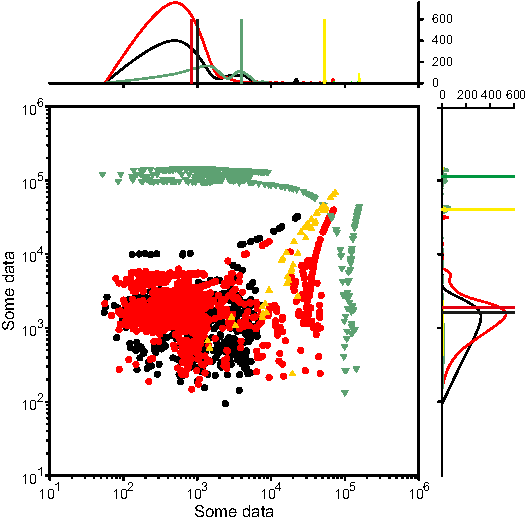
\includegraphics{./figure01.pdf}
\caption{Figure 1}
\end{figure}

And you can have it referenced as a figure

\begin{quote}
\textbf{Box 1} To highlight of defining some key concepts in Open
science without disrupting the flow of the articles, you can use a quote
format.
\end{quote}

\section*{Discussion}\label{discussion}
\addcontentsline{toc}{section}{Discussion}

What do the results mean? How does your results fit to the current
literature? How do they compare to other similar studies?

\section*{Conclusions}\label{conclusions}
\addcontentsline{toc}{section}{Conclusions}

What is the take-home message from this article?

\section{Acknowledgement}\label{acknowledgement}

We acknowledge the support from \ldots{} and the contribution from
\ldots{}.

Use this section to acknowledge funding and resource contributions to
the project.
